\documentclass{beamer}
\usepackage{ctex} %注意这个宏包
\usepackage{color}
\usepackage{graphics,graphicx}
\usepackage{pstricks,pst-node,pst-tree}
\usetheme{Boadilla}
\usecolortheme{beaver}
\usepackage{pstricks}
\usepackage{pst-plot}
\CTEXoptions[today=old]
\setCJKmainfont[BoldFont={SimHei},ItalicFont={KaiTi}] {WenQuanYi Micro Hei Mono}
\title{Introduction to Hidden Markov Model\\ 隐式马尔可夫模型}
\author{严春伟}
\institute[PKUSZ]{
    互联网研发中心\\
}
\date{\today}

\begin{document}
% ------------- title page ----------------------------
%--- the titlepage frame -------------------------%
\begin{frame}
  \titlepage
\end{frame}

\begin{frame}
\frametitle{Outline}
\tableofcontents
\end{frame}

\section{Introduction}
\begin{frame}{Sepcifaction of an HMM}
    \begin{block}{States}
    N--number of states
    \begin{itemize}
    \item Q=$\{ q_1, q_2, \cdots, q_T \}$
    \end{itemize}
    \end{block}

    \begin{block}{Symbols}
    M -- number of symbols
    \begin{itemize}
    \item O=$\{ o_1, o_2, \cdots, o_T \}$
    \end{itemize}
    \end{block}
\end{frame}

\begin{frame}{Sepcifaction of an HMM}
    \begin{block}{Transition Probility}
        \begin{itemize}
        \item A - the state transition probability matrix
            \begin{itemize}
            \item $a_{ij} = P(q_{t+1} = j | q_{t}=i)$
            \end{itemize}
        \end{itemize}
    \end{block}

    \begin{block}{Observation Probability}
        \begin{itemize}
        \item B- observation probability distribution
            \begin{itemize}
            \item $b_j{(k)} = P(O_t=k|q_t=j)$
            \end{itemize}
        \end{itemize}
    \end{block}
    
    \begin{block}{Initial State Distribution}
        \begin{itemize}
        \item $\pi$ -- the initial state distribution
        \end{itemize}
    \end{block}
\end{frame}

\begin{frame}{Sepcifaction of an HMM}
\begin{itemize}
\item Full HMM is thus specified as a triplet:
    \begin{itemize}
    \item $\lambda = (N,M,A,B,\pi)$
    \end{itemize}
\end{itemize}
\end{frame}

\section{A concrete example}
\begin{frame}{A concrete example}
    \begin{block}{Case Description}
        \begin{itemize}
        \item Alice and Bob, who live far apart from each other
        \item Bom is only interested in three activities: walk, shop,clean.
        \item Bom's choice is exclusively based on the weather.
        \item Alice tries to guess what the weather is like there.
        \end{itemize}
    \end{block}
\end{frame}

\begin{frame}{A concrete example}
    \begin{center}
    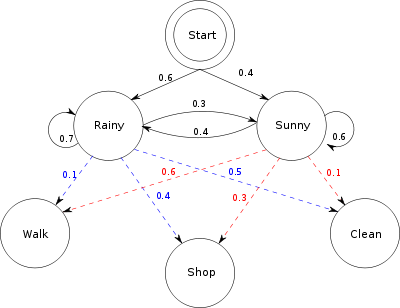
\includegraphics[height=150pt]{400px-HMMGraph.svg.png}
    \end{center}
\end{frame}

\begin{frame}{A concrete example}
    \begin{center}
    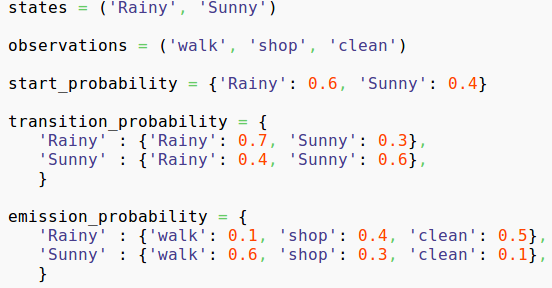
\includegraphics[height=130pt]{hmm-python.png}
    \end{center}
\end{frame}

\begin{frame}{A concrete example}
    \begin{block}{Find the Most Likely Sequence of Hidden States}
    \begin{itemize}
    \item get Bom's activities : $\{ walk, walk, clean, run  \}$
    \item trying to guess the most likely weather sequence there
    \end{itemize}

    \end{block}
\end{frame}

\section{Centroal Problems in HMM modeling}





\end{document}

